\section*{12 : Patrón Refactorización}
\label{sec:pr}
\addcontentsline{toc}{section}{\nameref{sec:pr}}


En este capítulo se analizará el proceso de resolver un problema mediante la aplicación de patrones de diseño de una forma evolutiva. Es decir, un primer diseño de corte será utilizado para la solución inicial, y luego esta solución será examinada y diversos patrones de diseño se aplicarán al problema (algunos de los cuales funcionaran y otros no). La pregunta clave que siempre se preguntó en la búsqueda de soluciones mejoradas es “¿qué va a cambiar?"     \newline

Este proceso es similar a lo que Martin Fowler habla en su libro \textit{Refactoring:Improving the Design of Existing Code\footnote{Addison-Wesley, 1999.}} (a pesar de que tiende a hablar de piezas de código más de diseños a nivel de patrón). 
Se comienza con una solución, y luego cuando se descubre que no es continuo en la satisfacción de sus necesidades, lo arregla. Por supuesto, esta es una tendencia natural, pero en la programación informática que ha sido muy difícil de lograr con programas de procedimiento, y la aceptación de la idea de que \textit{podemos} refactorizar código y añadir diseño al cuerpo de prueba como la programación orientada a objetos es "una cosa buena." \newline



\subsection*{Simulando el reciclador de basura}
\label{subsec:serdb}
\addcontentsline{toc}{subsection}{\nameref{subsec:serdb}}

La naturaleza de este problema es que la basura se lanza sin clasificar en un solo compartimiento, por lo que la información de tipo específico se pierde. Pero más tarde, la información de tipo específico debe ser recuperada para ordenar adecuadamente la basura. En la solución inicial, RTTI (descrito en el capítulo 12 de \textit{Thinking in Java, Segunda edición}) es utilizado.    \newline

Esto no es un diseño trivial, ya que tiene una restricción añadida. Eso es lo que hace que sea interesante — se parece más a los problemas desordenados que es probable que encuentre en su trabajo. La restricción adicional es que la basura llega a la planta de reciclaje del vertedero sanitario. El programa debe modelar la clasificación de esa basura. Aquí es donde entra en juego RTTI : usted tiene un montón de piezas anónimas de basura, y el programa se da cuenta exactamente de qué tipo son.  \newline


\begin{lstlisting} 
# c12:recyclea:RecycleA.py  
# Recycling with RTTI. 

class Trash: 
  private double weight 
  def __init__(self, double wt): weight = wt  
  abstract double getValue() 
  double getWeight(): return weight  
  # Sums the value of Trash in a bin: 
  static void sumValue(Iterator it): 
    double val = 0.0f 
    while(it.hasNext()): 
      # One kind of RTTI: 
      # A dynamically-checked cast 
      Trash t = (Trash)it.next() 
      # Polymorphism in action: 
      val += t.getWeight() * t.getValue() 
      print ( 
        "weight of " + 
        # Using RTTI to get type 
        # information about the class: 
        t.getClass().getName() + 
        " = " + t.getWeight()) 
        
    print "Total value = " + val 
    
class Aluminum(Trash): 
  static double val  = 1.67f 
  def __init__(self, double wt): .__init__(wt)  
  double getValue(): return val  
  static void setValue(double newval): 
    val = newval 
    
class Paper(Trash): 
  static double val = 0.10f 
  def __init__(self, double wt): .__init__(wt)  
  double getValue(): return val  
  static void setValue(double newval): 
    val = newval 
    
class Glass(Trash): 
  static double val = 0.23f 
  def __init__(self, double wt): .__init__(wt)  
  double getValue(): return val  
  static void setValue(double newval): 
    val = newval 
    
class RecycleA(UnitTest): 
  Collection  
    bin = ArrayList(), 
    glassBin = ArrayList(), 
    paperBin = ArrayList(), 
    alBin = ArrayList() 
  def __init__(self): 
    # Fill up the Trash bin: 
    for(int i = 0 i < 30 i++) 
      switch((int)(Math.random() * 3)): 
        case 0 : 
          bin.add(new 
            Aluminum(Math.random() * 100)) 
          break 
        case 1 : 
          bin.add(new 
            Paper(Math.random() * 100)) 
          break 
        case 2 : 
          bin.add(new 
            Glass(Math.random() * 100)) 
            
        def test(self): 
    Iterator sorter = bin.iterator() 
    # Sort the Trash: 
    while(sorter.hasNext()): 
      Object t = sorter.next() 
      # RTTI to show class membership: 
      if(t instanceof Aluminum) 
        alBin.add(t) 
      if(t instanceof Paper) 
        paperBin.add(t) 
      if(t instanceof Glass) 
        glassBin.add(t)   
        
    Trash.sumValue(alBin.iterator()) 
    Trash.sumValue(paperBin.iterator()) 
    Trash.sumValue(glassBin.iterator()) 
    Trash.sumValue(bin.iterator()) 
    
  def main(self, String args[]): 
    RecycleA().test() 
    
# :~ 
\end{lstlisting}

En los listados de código fuente disponibles para este libro, este archivo se colocará en el subdirectorio \textbf{recyclea} que se ramifica desde el subdirectorio \textbf{c12} (para el Capítulo 12). La herramienta de desembalaje se encarga de colocarlo en el subdirectorio correcto. La razón para hacer esto es que este capítulo reescribe este ejemplo particular, un número de veces y poniendo cada versión en su propio directorio (utilizando el paquete por defecto en cada directorio para que al ser invocado, el programa sea fácil), los nombres de clase no entren en conflicto.     \newline

Varios objetos \textbf{ArrayList} se crean para mantener referencias \textbf{Trash}. Claro, \textbf{ArrayList}s en realidad tendrá \textbf{Object}s vacíos (no sostendrán nada en absoluto). La razón por la que tienen \textbf{Trash} (o algo derivado de \textbf{Trash}) es sólo porque usted ha sido cuidadoso de no poner nada, excepto \textbf{Trash}. Si usted ha puesto algo “equivocado" en el \textbf{ArrayList}, usted no conseguirá ninguna compilación — advertencias de tiempo o errores — usted descubrirá sólo a través de una excepción, el tiempo de ejecución.   \newline

Cuando las referencias \textbf{Trash} son añadidas, pierden sus identidades específicas y se vuelven simplemente \textbf{Object reference}s (son \textit{upcast}). Sin embargo, debido al polimorfismo el comportamiento apropiado se sigue produciendo cuando los métodos dinámicamente enlazados son llamados a través de la \textbf{Iterator sorter}, una vez que el \textbf{Object} resultante haya sido lanzado de nuevo a \textbf{Trash. sumValue( )} también toma un \textbf{Iterator} para realizar operaciones en cada objeto en el \textbf{ArrayList}.   \newline

Parece una tontería moldear los tipos de \textbf{Trash} en una base de contenedor tipo referencia base, y luego dar un giro y abatirlo. ¿Por qué no poner la basura en el recipiente adecuado en el primer lugar? (De hecho, se trata de todo el enigma del reciclaje). En este programa sería fácil reparar, pero a veces la estructura y la flexibilidad de un sistema pueden beneficiarse enormemente de \textbf{downcasting}.     \newline

El programa cumple con los requisitos de diseño: funciona. Esto podría estar bien, siempre y cuando se trate de una solución de primera mano. Ahora bien, un programa útil tiende a evolucionar con el tiempo, por lo que se debe preguntar: “¿Qué pasa si la situación cambia?" Por ejemplo, el cartón es ahora un valioso producto reciclable, así que cómo eso será integrado en el sistema (especialmente si el programa es grande y complicado). Desde la anterior codificación de tipo de verificación en la declaración \textbf{switch} podría estar dispersa en todo el programa, usted debe ir a buscar todo ese código cada vez que se agrega un nuevo tipo, y si se le pasa alguna, el compilador no le dará ninguna ayuda señalando un error.  \newline

La clave para el mal uso de RTTI aquí, es que \textit{cada tipo se pone a prueba}. Si usted está buscando sólo un subconjunto de tipos, porque ese subconjunto necesita un tratamiento especial, eso probablemente está muy bien. Pero si usted está buscando para cada tipo dentro de una sentencia switch, entonces usted está probablemente perdiendo un punto importante, y definitivamente hacer su código menos mantenible. En la siguiente sección vamos a ver cómo este programa ha evolucionado a lo largo de varias etapas para llegar a ser mucho más flexible. Esto debe resultar un ejemplo valioso en el diseño del programa.     \newline



\subsection*{Mejorando el diseño}
\label{subsec:med}
\addcontentsline{toc}{subsection}{\nameref{subsec:med}}



Las soluciones en \textit{Design Patterns} se organizan en torno a la pregunta “¿Qué va a cambiar a medida que evoluciona este programa?" Esta suele ser la pregunta más importante que usted puede preguntar acerca de cualquier diseño. Si usted puede construir su sistema en torno a la respuesta, los resultados serán de dos vertientes: no sólo que su sistema permite un fácil (y barato) mantenimiento, sino que también se puedan producir componentes reutilizables, de modo que los otros sistemas se puedan construir de forma más económica. Esta es la promesa de la programación orientada a objetos, pero esto no sucede automáticamente; se requiere el pensamiento y la visión de su parte. En esta sección veremos cómo este proceso puede suceder durante el refinamiento de un sistema.    \newline

%  insight == visión, perspicacia.

A la pregunta “¿Qué va a cambiar? para el sistema de reciclaje es una respuesta común: se añadirán más tipos al sistema. El objetivo del diseño, entonces, es hacer de esta adición de tipos lo menos doloroso posible. En el programa de reciclaje, nos gustaría encapsular todos los lugares donde se menciona la información de tipo específico, así (si no por otra razón) los cambios se pueden localizar a esas encapsulaciones. Resulta que este proceso también limpia el resto del código considerablemente.  \newline

\subsubsection*{“Hacer más objetos"}
\label{subsubsec:med}
\addcontentsline{toc}{subsubsection}{\nameref{subsubsec:med}}


% ludicrously == ridículamente
Esto por lo general nos lleva a los principios de la programación orientada a objetos, la cual escuché por primera vez a Grady Booch: “Si el diseño es demasiado complicado, hacer más objetos." Esto es ridículamente simple y al mismo tiempo intuitivo; sin embargo es la guía más útil que he encontrado. (Es posible observar que "hacer más objetos" a menudo es equivalente a "agregar otro nivel de indirección.") En general, si usted encuentra un lugar con código desordenado, tenga en cuenta qué tipo de clase limpiaría eso. A menudo, el efecto secundario de la limpieza del código será un sistema que tiene mejor estructura y es más flexible.    \newline

Considere primero el lugar donde se crean los objetos \textbf{Trash}, que es una sentencia \textbf{switch} dentro de \textbf{main()}:    \newline

\begin{lstlisting} 
for(int i = 0 i < 30 i++) 
  switch((int)(Math.random() * 3)): 
    case 0 : 
      bin.add(new 
        Aluminum(Math.random() * 100)) 
      break 
    case 1 : 
      bin.add(new 
        Paper(Math.random() * 100)) 
      break 
    case 2 : 
        bin.add(new 
            Glass(Math.random() * 100)) 
\end{lstlisting}

Esto es definitivamente desordenado, y también un lugar donde usted debe cambiar el código cada vez que se agrega un nuevo tipo. Si comúnmente se añaden nuevos tipos, una mejor solución es un sólo método que toma toda la información necesaria y produce una referencia a un objeto del tipo correcto, ya proyectado a un objeto de basura. En \textit{Design Patterns} esto se conoce en general como un patrón creacional (de los cuales hay varios). El patrón específico que se aplicará aquí es una variante del \textit{Factory Method} (método fábrica). Aquí, el método fábrica es un miembro \textbf{static} de \textbf{Trash}, pero más comúnmente es un método que se anula en la clase derivada.  \newline

La idea del método de fábrica es que se le pasa la información esencial que necesita saber para crear su objeto, a continuación, retroceder y esperar por la referencia (ya upcast al tipo base) para que salga como el valor de retorno.  A partir de entonces, usted trata al objeto polimórficamente. Así, usted ni siquiera necesita saber el tipo exacto de objeto que se crea. De hecho, el método de fábrica lo esconde de usted para evitar el mal uso accidental. Si desea utilizar el objeto sin polimorfismo, debe utilizar explícitamente RTTI y difusión.    \newline

Pero hay un pequeño problema, especialmente cuando se utiliza el enfoque más complicado (no se muestra aquí) de hacer que el método de fábrica en la clase base y anulando en las clases derivadas. ¿Qué pasa si la información requerida en la clase derivada requiere más o diferentes argumentos? “la creación de más objetos" resuelve este problema. Para implementar el método de fábrica, la clase \textbf{Trash} consigue un nuevo método llamado \textbf{factory}. Para ocultar los datos creacionales, hay una nueva clase llamada \textbf{Messenger} que lleva toda la información necesaria para el método \textbf{factory} para crear el objeto \textbf{Trash} apropiado (hemos empezado haciendo referencia a \textit{Messenger} como un patrón de diseño, pero es bastante simple como para que no lo pueda elevar a ese estado). Aquí esta una simple implementación de \textbf{Messenger}:     \newline

\begin{lstlisting}
class Messenger: 
  int type 
  # Must change this to add another type: 
  static final int MAX_NUM = 4 
  double data 
  def __init__(self, int typeNum, double val): 
    type = typeNum % MAX_NUM 
    data = val 
\end{lstlisting}

El único trabajo de un objeto \textbf{Messenger} es mantener la información para el método \textbf{factory( )}. Ahora, si hay una situación en la que \textbf{factory( )} necesita información más o diferente para crear un nuevo tipo de objeto \textbf{Trash}, la interfaz \textbf{factory( )} no necesita ser cambiada. La clase \textbf{Messenger} puede ser cambiada mediante la adición de nuevos datos y nuevos constructores, o en la más típica manera de las subclases en la programación orientada a objetos.   \newline

El método \textbf{factory( )} para este sencillo ejemplo se ve así:     \newline

\begin{lstlisting}
static Trash factory(Messenger i): 
    switch(i.type): 
      default: # To quiet the compiler 
      case 0: 
        return Aluminum(i.data) 
      case 1: 
        return Paper(i.data) 
      case 2: 
        return Glass(i.data) 
      # Two lines here: 
      case 3:  
        return Cardboard(i.data)
\end{lstlisting}

Aquí, la determinación del tipo exacto de objeto es simple, pero se puede imaginar un sistema más complicado en el cual \textbf{factory( )} utiliza un algoritmo elaborado. El punto es que está ahora escondido en un lugar, y usted debe saber llegar a este lugar cuando se agregan nuevos tipos.  \newline

La creación de nuevos objetos es ahora mucho más simple en \textbf{main( )}:    \newline

\begin{lstlisting} 
    for(int i = 0 i < 30 i++) 
      bin.add( 
        Trash.factory( 
          Messenger( 
            (int)(Math.random() * Messenger.MAX_NUM), 
            Math.random() * 100))) 
\end{lstlisting}

Se crea un objeto \textbf{Messenger} para pasar los datos en \textbf{factory( )},
que a su vez produce una especie de objeto \textbf{Trash} en la pila y devuelve la referencia que se agrega al \textbf{ArrayList bin}. Claro, si cambia la cantidad y tipo de argumento, esta declaración todavía necesitará ser modificada, pero que puede ser eliminada si la creación del objeto \textbf{Messenger} está automatizada. Por ejemplo, un \textbf{ArrayList} de argumentos puede ser pasado en el constructor de un objeto \textbf{Messenger} (o directamente en una llamada \textbf{factory( )}, para el caso). Esto requiere que los argumentos sean analizados y verificados en tiempo de ejecución, pero proporciona la mayor flexibilidad.    \newline

Se puede ver en el código que el problema “vector de cambio" de la fábrica es responsable de resolver: si agrega nuevos tipos al sistema (el cambio), o el único código que debe ser modificado está dentro de la fábrica, por lo que la fábrica aísla el efecto de ese cambio. \newline


\subsection*{Un patrón para la creación de prototipos}
\label{subsec:upplcdp}
\addcontentsline{toc}{subsection}{\nameref{subsec:upplcdp}}

Un problema con el diseño anterior es que aún se requiere una ubicación central donde deben ser conocidos todos los tipos de los objetos: dentro del método \textbf{factory()}. Si regularmente se agregan nuevos tipos al sistema, el método \textbf{factory( )} debe cambiarse para cada nuevo tipo. Cuando se descubre algo como esto, es útil para tratar de avanzar un paso más y mover \textit{toda} la información sobre el tipo — incluyendo su creación — en la clase que representa este tipo. De esta manera, la única cosa que necesita hacer para agregar un nuevo tipo al sistema es heredar una sola clase.   \newline

Para mover la información relativa a la creación de tipo en cada tipo específico de \textbf{Trash}, se utilizará el patrón \textit{prototype} (del libro \textit{Design Patterns}). La idea general es que se tenga una secuencia principal de los objetos, uno de cada tipo que usted está interesado en hacer. Los objetos en esta secuencia \textit{sólo} se utilizan para la fabricación de nuevos objetos, utilizando una operación que no es diferente del esquema \textbf{clone( )} incorporado en la clase raíz \textbf{Object} de Java. En este caso, vamos a nombrar el método de clonación \textbf{tClone( )}. Cuando se esté listo para hacer un nuevo objeto, presumiblemente se tiene algún tipo de información que establece el tipo de objeto que se desea crear, a continuación se mueve a través de la secuencia maestra comparando su información con cualquier información apropiada que se encuentra en los objetos de prototipo en la secuencia principal. Cuando se encuentra uno que se ajuste a sus necesidades, se clona.    \newline

En este esquema no hay información modificable para la creación. Cada objeto sabe cómo exponer la información adecuada y la forma de clonarse a sí mismo. Así, el método \textbf{factory( )} no necesita ser cambiado cuando se añade un nuevo tipo al sistema.     \newline

Un enfoque al problema del prototipado es agregar un número de métodos para apoyar la creación de nuevos objetos. Ahora bien, en Java 1.1 ya hay apoyo para la creación de nuevos objetos si tiene una referencia al objeto \textbf{Class}. Con Java 1.1 \textit{reflection (reflexión)} (introducido en el capítulo 12 de \textit{Thinking in Java}, segunda edición) puede llamar a un constructor, incluso si tiene sólo una referencia al objeto \textbf{Class}. Esta es la solución perfecta para el problema del prototipado.   \newline

La lista de los prototipos será representada indirectamente por una lista de referencias a todos los objetos de \textbf{Class} que se desea crear. En adición, si el prototipado falla, el método \textbf{factory( )} asumirá que es porque un objeto particular \textbf{Class} no estaba en la lista, y se tratará de cargarlo. Al cargar los prototipos de forma dinámica como este, la clase \textbf{Trash} no necesita saber con qué tipos está trabajando, por lo que no necesita ninguna modificación al agregar nuevos tipos. Esto permite que sea fácilmente reutilizable durante todo el resto del capítulo.     \newline

\begin{lstlisting} 
# c12:trash:Trash.py 
# Base class for Trash recycling examples. 

class Trash: 
  private double weight 
  def __init__(self, double wt): weight = wt  
  def __init__(self): 
  def getValue(self) 
  def getWeight(self): return weight  
  # Sums the value of Trash given an 
  # Iterator to any container of Trash: 
  def sumValue(self, Iterator it): 
    double val = 0.0f 
    while(it.hasNext()): 
      # One kind of RTTI: 
      # A dynamically-checked cast 
      Trash t = (Trash)it.next() 
      val += t.getWeight() * t.getValue() 
      print ( 
        "weight of " + 
        # Using RTTI to get type 
        # information about the class: 
        t.getClass().getName() + 
        " = " + t.getWeight()) 
        
    print "Total value = " + val 
    
  # Remainder of class provides  
  # support for prototyping: 
  private static List trashTypes =  
    ArrayList() 
  def factory(self, Messenger info): 
    for(int i = 0 i < len(trashTypes) i++): 
      # Somehow determine the type 
      # to create, and create one: 
      Class tc = (Class)trashTypes.get(i) 
      if (tc.getName().index(info.id) != -1): 
        try: 
          # Get the dynamic constructor method 
          # that takes a double argument: 
          Constructor ctor = tc.getConstructor( 
              Class[]{ double.class ) 
          # Call the constructor   
          # to create a object: 
          return (Trash)ctor.newInstance( 
            Object[]{Double(info.data)) 
         catch(Exception ex): 
          ex.printStackTrace(System.err) 
          throw RuntimeException( 
            "Cannot Create Trash") 
            
    # Class was not in the list. Try to load it, 
    # but it must be in your class path! 
    try: 
      print "Loading " + info.id 
      trashTypes.add(Class.forName(info.id)) 
     catch(Exception e): 
      e.printStackTrace(System.err) 
      throw RuntimeException( 
        "Prototype not found") 
        
    # Loaded successfully.  
    # Recursive call should work: 
    return factory(info) 
    
  public static class Messenger: 
    public String id 
    public double data 
    public Messenger(String name, double val): 
      id = name 
      data = val 
      
# :~ 
\end{lstlisting}

La clase básica \textbf{Trash} y \textbf{sumValue( )} permanecen como antes. El resto de la clase soporta el patrón de prototipado. Primero ve dos clases internas (que se hacen \textbf{static}, así que son las clases internas solamente para los propósitos de la organización de código) describiendo excepciones que pueden ocurrir. Esto es seguido por un  \textbf{ArrayList} llamado \textbf{trashTypes}, que se utiliza para mantener las referencias \textbf{Class}.    \newline

En \textbf{Trash.factory( )}, el \textbf{String} dentro del objeto \textbf{Messenger} \textbf{id} (una versión diferente de la clase \textbf{Messenger} que el de la discusión previa) contiene el nombre del tipo de la \textbf{Trash} a crearse; este \textbf{String} es comparado con los nombres \textbf{Class} en la lista. Si hay una coincidencia, entonces ese es el objeto a crear. Por supuesto, hay muchas formas para determinar qué objeto se desea hacer. Éste se utiliza para que la información leída desde un archivo se pueda convertir en objetos.    \newline

Una vez que se haya descubierto qué tipo de \textbf{Trash} se va a crear, a continuación, los métodos de reflexión entran en juego. El método \textbf{getConstructor( )} toma un argumento que es un array de referencias \textbf{Class}. Este array representa los argumentos, en su debido orden, para el constructor que se está buscando. Aquí, el array es creado de forma dinámica usando Java 1.1 la sintaxis para la creación de los arrays es:  \newline

\begin{lstlisting} 
Class[]:double.class
\end{lstlisting}

Este código asume que cada tipo \textbf{Trash} tiene un constructor que toma un \textbf{double} (y observe que \textbf{double.class} es distinto de \textbf{Double.class}). También es posible, por una solución más flexible, llamar \textbf{getConstructors( )}, que devuelve un array con los posibles constructores.  \newline

Lo que devuelve \textbf{getConstructor( )} es una referencia a un objeto \textbf{Constructor} (parte de \textbf{java.lang.reflect}). El constructor se llama de forma dinámica con el método \textbf{newInstance( )}, lo cual toma un array de \textbf{Object} conteniendo los argumentos reales. Este array se crea de nuevo utilizando la sintaxis de Java 1.1, así:    \newline

\begin{lstlisting} 
Object[]{Double(Messenger.data)
\end{lstlisting}

En este caso, sin embargo, el \textbf{double} debe ser colocado dentro de una clase de contenedor de modo que pueda ser parte de este array de objetos. El proceso de llamar \textbf{newInstance( )} extrae el \textbf{double}, pero se puede ver que es un poco confuso — un argumento puede ser un \textbf{double} o un \textbf{Double}, pero cuando se hace la llamada siempre se debe pasar en un \textbf{Double}. Afortunadamente, existe este problema sólo para los tipos primitivos.   \newline

Una vez se entienda cómo hacerlo, el proceso de crear un nuevo objeto dado sólo una referencia \textbf{Class} es muy simple. Reflexión también le permite llamar métodos en esta misma manera dinámica.      \newline

Por supuesto, la referencia apropiada \textbf{Class} podría no estar en la lista \textbf{trashTypes}. En este caso, el \textbf{return} en el bucle interno no se ejecuta y se retirará al final. Aquí, el programa trata de rectificar la situación mediante la carga del objeto \textbf{Class} dinámicamente y agregarlo a la lista \textbf{trashTypes}. Si aún así no se puede encontrar algo anda realmente mal, pero si la carga tiene éxito, entonces el método  \textbf{factory} se llama de forma recursiva para volver a intentarlo.    \newline

Tal como se muestra, la belleza de este diseño es que el código no necesita ser cambiado, independientemente de las diferentes situaciones en que se utilice (asumiendo que todas las subclases \textbf{Trash} contiene un constructor que toma un solo argumento \textbf{double}).     \newline


\subsection*{Subclases \textbf{Trash}}
\label{subsec:st}
\addcontentsline{toc}{subsection}{\nameref{subsec:st}}


Para encajar en el esquema de prototipado, lo único que se requiere de cada nueva subclase de \textbf{Trash} es que contiene un constructor que toma un argumento \textbf{double}. Java, reflexión se encarga de todo lo demás.    \newline

Éstos son los diferentes tipos de \textbf{Trash}, cada uno en su propio archivo, pero parte del paquete \textbf{Trash} (de nuevo, para facilitar la reutilización dentro del capítulo) es:       \newline

\begin{lstlisting} 
# c12:trash:Aluminum.py  
# The Aluminum class with prototyping. 

class Aluminum(Trash): 
  private static double val = 1.67f 
  def __init__(self, double wt): .__init__(wt)  
  def getValue(self): return val  
  def setValue(self, double newVal): 
    val = newVal 
    
# :~ 
# c12:trash:Paper.py  
# The Paper class with prototyping. 

class Paper(Trash): 
  private static double val = 0.10f 
  def __init__(self, double wt): .__init__(wt)  
  def getValue(self): return val  
  def setValue(self, double newVal): 
    val = newVal 
    
# :~ 
# c12:trash:Glass.py  
# The Glass class with prototyping.

class Glass(Trash): 
  private static double val = 0.23f 
  def __init__(self, double wt): .__init__(wt)  
  def getValue(self): return val  
  def setValue(self, double newVal): 
    val = newVal 
    
# :~ 
\end{lstlisting}

Y aquí se muestra un nuevo tipo de \textbf{Trash}(basura):

\begin{lstlisting} 
# c12:trash:Cardboard.py  
# The Cardboard class with prototyping. 

class Cardboard(Trash): 
  private static double val = 0.23f 
  def __init__(self, double wt): .__init__(wt)  
  def getValue(self): return val  
  def setValue(self, double newVal): 
    val = newVal 
    
# :~ 
\end{lstlisting}

Se puede ver que, aparte del constructor, no hay nada de especial en cualquiera de estas clases.


\subsection*{Analizar \textbf{Trash} desde un archivo externo}
\label{subsec:atduae}
\addcontentsline{toc}{subsection}{\nameref{subsec:atduae}}


La información sobre los objetos \textbf{Trash} será leído desde un archivo exterior. El archivo cuenta con toda la información necesaria sobre cada pieza de \textbf{Trash} en una sola línea en la forma de \textbf{Trash:weight}, como:     \newline

\begin{lstlisting} 
# c12:trash:Trash.dat 
c12.trash.Glass:54 
c12.trash.Paper:22 
c12.trash.Paper:11 
c12.trash.Glass:17 
c12.trash.Aluminum:89 
c12.trash.Paper:88 
c12.trash.Aluminum:76 
c12.trash.Cardboard:96 
c12.trash.Aluminum:25 
c12.trash.Aluminum:34 
c12.trash.Glass:11 
c12.trash.Glass:68 
c12.trash.Glass:43 
c12.trash.Aluminum:27 
c12.trash.Cardboard:44 
c12.trash.Aluminum:18 
c12.trash.Paper:91 
c12.trash.Glass:63 
c12.trash.Glass:50 
c12.trash.Glass:80 
c12.trash.Aluminum:81 
c12.trash.Cardboard:12 
c12.trash.Glass:12 
c12.trash.Glass:54 
c12.trash.Aluminum:36 
c12.trash.Aluminum:93 
c12.trash.Glass:93 
c12.trash.Paper:80 
c12.trash.Glass:36 
c12.trash.Glass:12 
c12.trash.Glass:60 
c12.trash.Paper:66 
c12.trash.Aluminum:36 
c12.trash.Cardboard:22 
# :~ 
\end{lstlisting}

Tenga en cuenta que la ruta de la clase debe ser incluida al dar los nombres de las clases, de lo contrario la clase no será encontrada.\newline

Este archivo se lee utilizando la herramienta \textbf{StringList} definida previamente, y cada línea se selecciona de forma independiente usando el método \textbf{String indexOf( )} para producir el índice del ‘:’. Esto se utiliza primero con el método \textbf{String substring( )} para extraer el nombre del tipo de \textbf{Trash}, y seguidamente se obtiene el valor convertido en \textbf{double} con el método \textbf{static Double.valueOf( )}. El método \textbf{trim( )}  elimina los espacios en blanco en ambos extremos de un string : cadena. \newline

El analizador sintáctico de \textbf{Trash } es colocado en un archivo separado, ya que se reutilizará en todo este capítulo: \newline

\begin{lstlisting} 
# c12:trash:ParseTrash.py  
# Parse file contents into Trash objects, 
# placing each into a Fillable holder. 

class ParseTrash: 
  def fillBin(String filename, Fillable bin): 
    for line in open(filename).readlines(): 
      String type = line.substring(0,  
        line.index(':')).strip() 
      double weight = Double.valueOf( 
        line.substring(line.index(':') + 1) 
          .strip()).doubleValue() 
      bin.addTrash( 
        Trash.factory( 
          Trash.Messenger(type, weight))) 
          
  # Special case to handle Collection: 
  def fillBin(String filename, Collection bin): 
    fillBin(filename, FillableCollection(bin)) 
    
    # :~
\end{lstlisting}

En \textbf{RecycleA.py}, un \textbf{ArrayList} se utiliza para contener los objetos \textbf{Trash}. Sin embargo, otros tipos de contenedores pueden ser utilizados también. Para permitir esto, la primera versión de \textbf{fillBin( )} hace una referencia a un \textbf{Fillable}, lo cual es simplemente una \textbf{interface} que soporta un método llamado \textbf{addTrash( )}:     \newline

\begin{lstlisting} 
# c12:trash:Fillable.py  
# Any object that can be filled with Trash.

class Fillable: 
  def addTrash(self, Trash t) 
# :~ 
\end{lstlisting}

Cualquier cosa que soporta esta interfaz se puede utilizar con \textbf{fillBin}. Claro, \textbf{Collection} no implementa \textbf{Fillable}, por lo que no va a funcionar. Dado que \textbf{Collection} se utiliza en la mayoría de los ejemplos, tiene sentido añadir un segundo método \textbf{fillBin( )} sobrecargado que toma un \textbf{Collection}. Cualquier \textbf{Collection} a continuación, se puede utilizar como un objeto \textbf{Fillable} usando una clase adaptador así:   \newline

\begin{lstlisting} 
# c12:trash:FillableCollection.py  
# Adapter that makes a Collection Fillable. 

class FillableCollection(Fillable): 
  private Collection c 
  def __init__(self, Collection cc):  
    c = cc  
    
  def addTrash(self, Trash t): 
    c.add(t) 
    
# :~ 
\end{lstlisting}

Se puede ver que el único trabajo de esta clase es conectar el método \textbf{addTrash( )} de \textbf{Fillable} a \textbf{Collection’s add( )}. Con esta clase en la mano, el método sobrecargado \textbf{fillBin( )}  se puede utilizar con un \textbf{Collection} en \textbf{ParseTrash.py}, como se muestra:   \newline

\begin{lstlisting} 
  public static void  
  fillBin(String filename, Collection bin): 
    fillBin(filename, FillableCollection(bin)) 
\end{lstlisting}

Este enfoque funciona para cualquier clase de contenedor que se utiliza con frecuencia. Alternativamente, la clase de contenedor puede proporcionar su propio adaptador que implementa \textbf{Fillable}. (Se verá esto después, en \textbf{DynaTrash.py.})     \newline



\subsection*{Reciclaje con prototipos}
\label{subsec:rcp}
\addcontentsline{toc}{subsection}{\nameref{subsec:rcp}}


Ahora se puede ver la versión revisada de \textbf{RecycleA.py} utilizando la técnica de prototipos, de tal forma que:     \newline

\begin{lstlisting} 
# c12:recycleap:RecycleAP.py  
# Recycling with RTTI and Prototypes. 

class RecycleAP(UnitTest): 
  Collection 
    bin = ArrayList(),  
    glassBin = ArrayList(), 
    paperBin = ArrayList(), 
    alBin = ArrayList() 
  def __init__(self): 
    # Fill up the Trash bin: 
    ParseTrash.fillBin( 
      "../trash/Trash.dat", bin) 
      
  def test(self): 
    Iterator sorter = bin.iterator() 
    # Sort the Trash: 
    while(sorter.hasNext()): 
      Object t = sorter.next() 
      # RTTI to show class membership: 
      if(t instanceof Aluminum) 
        alBin.add(t) 
      if(t instanceof Paper) 
        paperBin.add(t) 
      if(t instanceof Glass) 
        glassBin.add(t) 
        
    Trash.sumValue(alBin.iterator()) 
    Trash.sumValue(paperBin.iterator()) 
    Trash.sumValue(glassBin.iterator()) 
    Trash.sumValue(bin.iterator()) 
    
  def main(self, String args[]): 
    RecycleAP().test() 
    
# :~     
\end{lstlisting}

Todos los objetos \textbf{Trash}, así como las clases \textbf{ParseTrash} y de apoyo, ahora son parte del paquete de \textbf{c12.trash}, por lo que simplemente son importados.     \newline

El proceso de abrir el archivo de datos que contiene descripciones \textbf{Trash} y el análisis de ese archivo han sido envuelto en el método \textbf{static} \textbf{ParseTrash.fillBin( )}, por lo que ahora ya no es parte de nuestro enfoque de diseño. Se verá que en el resto del capítulo, no importa que se agreguen nuevas clases, \textbf{ParseTrash.fillBin( )} continuará funcionando sin cambios, lo que indica que es un buen diseño.   \newline

En términos de creación de objetos, este diseño en efecto, localiza severamente los cambios que necesita hacer para agregar un nuevo tipo al sistema. Ahora bien, hay un problema significativo en el uso de RTTI que se muestra claramente aquí. El programa parece funcionar bien, y sin embargo, nunca se detecta algún cardboard (cartón), a pesar de que cardboard está en la lista! Esto sucede debido al uso de RTTI, que busca sólo los tipos que le indican que debe buscar. La pista que RTTI está siendo mal utilizada es que cada tipo en el sistema se está probando, en lugar de un solo tipo o subconjunto de tipos. Como se verá más adelante, hay maneras de utilizar polimorfismo en lugar de estar probando cada tipo. Pero si usa RTTI mucho de esta manera, y añade un nuevo tipo a su sistema, usted puede olvidar fácilmente  hacer los cambios necesarios en su programa y producir un error difícil de encontrar. Así que vale la pena tratar de eliminar RTTI en este caso, no sólo por razones estéticas — se produce código más mantenible.      \newline



\subsection*{Haciendo abstracción de uso}
\label{subsec:hadu}
\addcontentsline{toc}{subsection}{\nameref{subsec:hadu}}


Con la creación fuera del camino, es el momento de abordar el resto del diseño: donde se utilizan las clases. Dado que es el acto de la clasificación en los contenedores que es particularmente feo y expuesto, por qué no tomar ese proceso y ocultarlo dentro de una clase? Este es el principio de "Si debe hacer algo feo, al menos localizar la fealdad dentro de una clase." Se parece a esto:   \newline

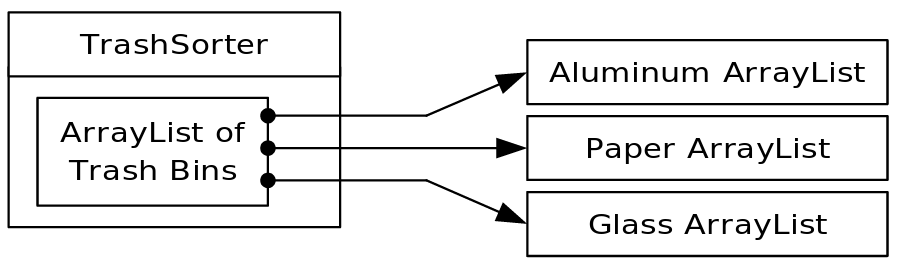
\includegraphics[width=\textwidth]{Pag147SinTraducir.png}

La inicialización de objetos \textbf{TrashSorter} ahora debe ser cambiado cada vez que un nuevo tipo de \textbf{Trash} se añade al modelo. Usted podría imaginar que la clase \textbf{TrashSorter} podría ser algo como esto:     \newline

\begin{lstlisting} 
class TrashSorter(ArrayList): 
  def sort(self, Trash t): /* ... */  
\end{lstlisting}

Es decir, \textbf{TrashSorter} es un \textbf{ArrayList} de referencias a \textbf{ArrayList}s de referencias \textbf{Trash}, y con \textbf{add()} se puede instalar otro, así:  \newline

\begin{lstlisting} 
TrashSorter ts = TrashSorter() 
ts.add(ArrayList()) 
\end{lstlisting}

Ahora, sin embargo, \textbf{sort( )} se convierte en un problema. ¿Cómo el método estático - codificado trata con el hecho de que un nuevo tipo ha sido añadido? Para solucionar esto, la información de tipo debe ser removido de \textbf{sort( )} de manera que todo lo que necesita hacer es llamar a un método genérico que se ocupa de los detalles de tipo. Esto, por supuesto, es otra manera de describir un método dinámicamente enlazado. Así \textbf{sort( )} simplemente se moverá a través de la secuencia y llamará a un método dinámicamente enlazado para cada \textbf{ArrayList}. Dado que el trabajo de este método es tomar las piezas de \textbf{Trash} en que está interesado, este es llamado \textbf{grab(Trash)}. La estructura ahora queda como:       \newline

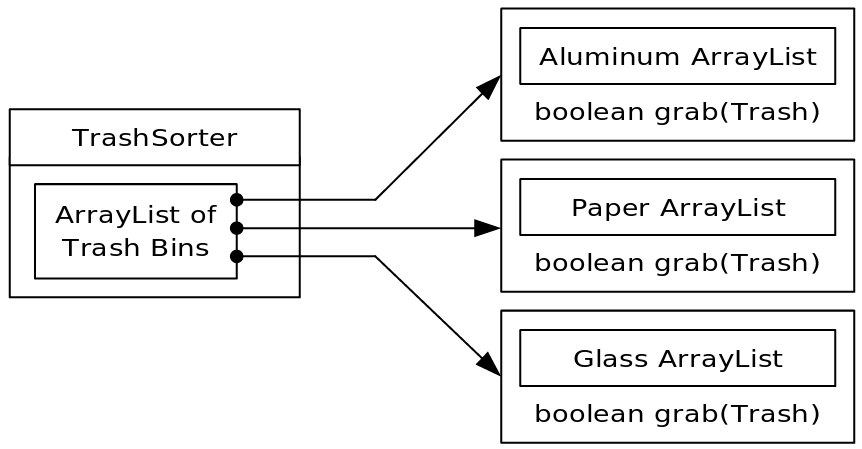
\includegraphics[width=\textwidth]{Pagina148SinTraducir.png}

\textbf{TrashSorter} necesita llamar cada método \textbf{grab()} y obtener un resultado diferente dependiendo de qué tipo de \textbf{Trash} \textbf{ArrayList} actual está sosteniendo. Es decir, cada \textbf{ArrayList} debe ser consciente del tipo que contiene. El enfoque clásico a este problema es crear una clase "\textbf{Trash bin} : Contenedor de basura" base y heredar una nueva clase derivada para cada tipo diferente que quiera mantener. Si Java tenía un mecanismo de tipo parametrizado ese probablemente sería el enfoque más sencillo. Pero en lugar de la codificación manual de todas las clases que tal mecanismo debe estar construyendo para nosotros, una mayor observación puede producir un mejor enfoque.   \newline

Un principio básico de diseño en programación orientada a objetos es: "Usar los miembros de datos para la variación en el estado, utilizar el polimorfismo para la variación en el comportamiento." Su primer pensamiento podría ser que el método \textbf{grab( )} ciertamente se comporta de manera diferente para un \textbf{ArrayList} que contiene \textbf{Paper} que por su parte contiene \textbf{Glass}. Pero lo que hace es estrictamente dependiente del tipo, y nada más. Esto podría interpretarse como un estado diferente, y dado que Java tiene una clase para representar el tipo \textbf{(Class)}, esto se puede utilizar para determinar el tipo de \textbf{Trash} que sostendrá a \textbf{Tbin} en particular .       \newline

El constructor para este \textbf{Tbin} requiere lo de la \textbf{Class} de su elección. Esto le dice al \textbf{ArrayList} qué tipo se supone que debe mantener. Entonces el método \textbf{grab( )} usa \textbf{Class BinType} y RTTI para ver si el objeto \textbf{Trash} que ha entregado coincide con el tipo que se supone que ha seleccionado.      \newline

Aquí esta una nueva versión del programa:       \newline

\begin{lstlisting} 
# c12:recycleb:RecycleB.py 
# Containers that grab objects of interest. 

# A container that admits only the right type 
# of Trash (established in the constructor): 
class Tbin: 
  private Collection list = ArrayList() 
  private Class type 
  def __init__(self, Class binType): type = binType  
  def grab(self, Trash t): 
    # Comparing class types: 
    if(t.getClass().equals(type)): 
      list.add(t) 
      return 1 # Object grabbed 
      
    return 0 # Object not grabbed  
    
  def iterator(self): 
    return list.iterator() 
    
class TbinList(ArrayList): 
  def sort(self, Trash t): 
    Iterator e = iterator() # Iterate over self 
    while(e.hasNext()) 
      if(((Tbin)e.next()).grab(t)) return 
    # Need a Tbin for this type: 
        add(Tbin(t.getClass())) 
    sort(t) # Recursive call 
    
class RecycleB(UnitTest): 
  Collection bin = ArrayList() 
  TbinList trashBins = TbinList() 
  def __init__(self): 
    ParseTrash.fillBin("../trash/Trash.dat",bin) 
    
  def test(self): 
    Iterator it = bin.iterator() 
    while(it.hasNext()) 
      trashBins.sort((Trash)it.next()) 
    Iterator e = trashBins.iterator() 
    while(e.hasNext()): 
      Tbin b = (Tbin)e.next() 
      Trash.sumValue(b.iterator()) 
      
    Trash.sumValue(bin.iterator()) 
    
  def main(self, String args[]): 
    RecycleB().test() 
    
# :~ 
\end{lstlisting}

\textbf{Tbin} contiene una referencia \textbf{Class} \textbf{type} que establece en el constructor qué tipo debe seleccionar. El método \textbf{grab()} revisa este tipo contra el objeto que se pasa. Tenga en cuenta que en este diseño, \textbf{grab()} solo acepta objetos \textbf{Trash} de este modo usted consigue la comprobación de tipos en tiempo de compilación del tipo base, pero también se podría aceptar solo \textbf{Object} y aún así funcionaría.      \newline

\textbf{TbinList} sostiene un conjunto de referencias \textbf{Tbin}, así que \textbf{sort()} puede iterar a través de los \textbf{Tbin}s cuando está buscando una pareja para el objeto \textbf{Trash} se lo ha transmitido. Si este no encuentra una pareja, crea un nuevo \textbf{Tbin} para el tipo que no ha sido enconstrado, y hace una llamada recursiva a sí mismo – la próxima vez encontrará el nuevo bin.
%   time around == vez

Note la generalidad de este código: no cambia en absoluto si se añaden nuevos tipos. Si la mayor parte de su código no necesita cambiar cuando se añade un nuevo tipo (o algún otro cambio ocurre) entonces usted tiene un sistema fácilmente extensible.

\newpage


\subsection*{Despacho múltiple}
\label{subsec:dmul}
\addcontentsline{toc}{subsection}{\nameref{subsec:dmul}}

El diseño anterior es ciertamente satisfactorio. La adición de nuevos tipos al sistema consiste en añadir o modificar clases distintas sin causar cambios en el código que se propaguen por todo el sistema. En adición, RTTI no está "mal utilizada" como lo estaba en \textbf{RecycleA.py}. Sin embargo, es posible ir un paso más allá y tomar un punto de vista purista sobre RTTI y decir que debe ser eliminada por completo de la operación de clasificar la basura en los contenedores. \newline

Para lograr esto, primero debe tomar la perspectiva de que todas las actividades de tipo dependiente — tal como la detección del tipo de un pedazo de \textbf{Trash} y ponerla en el recipiente apropiado — deben ser controladas a través del polimorfismo y de un enlace dinámico. \newline

Los ejemplos anteriores primero ordenados por tipo, luego actuando en las secuencias de elementos que eran todos de un tipo en particular. Pero cada vez que usted se encuentra eligiendo tipos particulares, deténgase y piense. 
Toda la idea de polimorfismo (dinámicamente enlazado con llamadas a métodos) es encargarse de la información de tipo específico para usted. Así que ¿por qué la búsqueda de tipos?      \newline

La respuesta es algo que probablemente no se piensa: que Python sólo realiza despacho individual. Es decir, si está realizando una operación en más de un objeto cuyo tipo es desconocido, Python invocará el mecanismo de enlace dinámico en sólo uno de esos tipos. Esto no resuelve el problema, así que se termina la detección de algunos tipos manualmente y produciendo eficazmente su propio comportamiento de enlace dinámico. \newline

La solución es llamada  \textit{multiple dispatching (Despacho múltiple)} lo cual significa la creación de una configuración tal que una única llamada al método produce más de una llamada a un método dinámico y por lo tanto determina más de un tipo en el proceso. Para conseguir este efecto, se necesita trabajar con más de una jerarquía de tipos: se necesitará una jerarquía de tipos para cada envío. En el siguiente ejemplo se trabaja con dos jerarquías: la familia \textbf{Trash} existente y una jerarquía de los tipos de contenedores de basura, en los cuales los desechos serán colocados. Esta segunda jerarquía no siempre es evidente y en este caso se requiere crear un orden para producir múltiples despachos (en este caso habrá sólo dos despachos, lo cual hace referencia como \textit{double dispatching (despacho doble)}).
% Despacho, envio (sinonimos)
\newpage


\subsubsection*{La implementación del despacho doble}
\label{subsubsec:liddd}
\addcontentsline{toc}{subsubsection}{\nameref{subsubsec:liddd}}


Recuerde que el polimorfismo puede ocurrir sólo a través de llamadas a métodos, así que si quiere que se produzca el despacho doble, deben existir dos llamadas a métodos: uno utilizado para determinar el tipo dentro de cada jerarquía. En la jerarquía \textbf{Trash} habrá un nuevo método llamado \textbf{addToBin()}, que toma un argumento de un array de \textbf{TypedBin}. Utiliza este array para recorrer y tratar de agregarse a sí misma al contenedor apropiado, y aquí es donde se verá el despacho doble. \newline

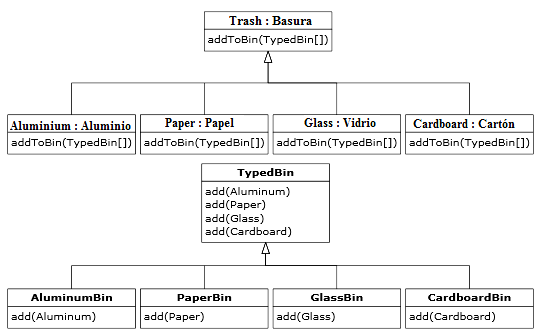
\includegraphics[width=\textwidth]{DobleDespacho}

\vspace{0.5 cm}

La nueva jerarquía es \textbf{TypedBin}, y que contiene su propio método llamado \textbf{add()} que también es utilizado polimórficamente. Pero aquí está un giro adicional: \textbf{add()} está sobrecargado  para tomar argumentos de los diferentes tipos de \textit{trash : basura}. Así que una parte esencial del esquema de doble despacho también implica una sobrecarga. El rediseño del programa produce un dilema: ahora es necesario para la clase base \textbf{Trash} contener un método \textbf{addToBin()}. Un enfoque consiste en copiar todo el código y cambiar la clase base. Otro enfoque, que puede tomar es cuando no se tiene el control del código fuente, es poner el método \textbf{addToBin( )} dentro de un \textbf{interface}, dejar \textbf{Trash} solo, y heredar nuevos tipos específicos de \textbf{Aluminum, Paper, Glass}, y \textbf{Cardboard}. Este es el enfoque que se tomará aquí.    \newline

La mayoría de las clases en este diseño debe ser \textbf{public}, por lo que se colocan en sus propios archivos. Aquí esta la interfaz:     \newline

\begin{lstlisting} 
# c12:doubledispatch:TypedBinMember.py 
# An class for adding the double  
# dispatching method to the trash hierarchy  
# without modifying the original hierarchy.

class TypedBinMember: 
  # The method: 
  boolean addToBin(TypedBin[] tb) 
# :~ 
\end{lstlisting}

En cada subtipo particular de \textbf{Aluminum, Paper, Glass} , and \textbf{Cardboard}, el método \textbf{addToBin( )} en la interfaz \textbf{interface TypedBinMember} es implementado, pero \textit{parece}  que el código es exactamente el mismo en cada caso:    \newline

\begin{lstlisting} 
# c12:doubledispatch:DDAluminum.py 
# Aluminum for double dispatching. 

class DDAluminum(Aluminum)  
    implements TypedBinMember: 
  def __init__(self, double wt): .__init__(wt)  
  def addToBin(self, TypedBin[] tb): 
    for(int i = 0 i < tb.length i++) 
      if(tb[i].add(self)) 
        return 1 
    return 0 
    
# :~ 
# c12:doubledispatch:DDPaper.py 
# Paper for double dispatching. 

class DDPaper(Paper)  
    implements TypedBinMember: 
  def __init__(self, double wt): .__init__(wt)  
  def addToBin(self, TypedBin[] tb): 
    for(int i = 0 i < tb.length i++) 
      if(tb[i].add(self)) 
        return 1 
    return 0 
    
# :~ 
# c12:doubledispatch:DDGlass.py 
# Glass for double dispatching. 

class DDGlass(Glass)  
    implements TypedBinMember: 

  def __init__(self, double wt): .__init__(wt)  
  def addToBin(self, TypedBin[] tb): 
    for(int i = 0 i < tb.length i++) 
      if(tb[i].add(self)) 
        return 1 
    return 0 
    
# :~ 
# c12:doubledispatch:DDCardboard.py 
# Cardboard for double dispatching. 

class DDCardboard(Cardboard)  
    implements TypedBinMember: 
  def __init__(self, double wt): .__init__(wt)  
  def addToBin(self, TypedBin[] tb): 
    for(int i = 0 i < tb.length i++) 
      if(tb[i].add(self)) 
        return 1 
    return 0 
    
# :~ 
\end{lstlisting}

El código en cada \textbf{addToBin( )} llama \textbf{add( )} para cada objeto \textbf{TypedBin} en el array. Pero notece el argumento: \textbf{this}. El tipo de \textbf{this} es diferente para cada subclase de \textbf{Trash}, por lo que el código es diferente. (Aunque este código se beneficiará si un mecanismo de tipo parametrizado es alguna vez agregado a Java.) Así que esta es la primera parte del doble despacho, porque una vez que está dentro de este método se sabe que es \textbf{Aluminum},  o \textbf{Paper}, etc. Durante la llamada a \textbf{add( )}, esta información se pasa a través del tipo de \textbf{this}. El compilador resuelve la llamada a la versión correcta sobrecargada de \textbf{add( )}. Pero desde que \textbf{tb[i]} produce una referencia al tipo base \textbf{TypedBin}, esta llamada va a terminar llamando a un método diferente dependiendo del tipo de \textbf{TypedBin} que está actualmente seleccionado. Ese es el segundo despacho. \newline

Aquí esta la clase base para \textbf{TypedBin}:         \newline

\begin{lstlisting} 
# c12:doubledispatch:TypedBin.py 
# A container for the second dispatch. 

class TypedBin: 
  Collection c = ArrayList() 
  def addIt(self, Trash t): 
    c.add(t) 
    return 1 
    
  def iterator(self): 
    return c.iterator() 
    
  def add(self, DDAluminum a): 
    return 0 
    
  def add(self, DDPaper a): 
    return 0 
    
  def add(self, DDGlass a): 
    return 0 
    
  def add(self, DDCardboard a): 
    return 0 
    
# :~ 
\end{lstlisting}

Se puede ver que todos los métodos sobrecargados \textbf{add( )} retornan  \textbf{false}. Si el método no está sobrecargado en una clase derivada, continuará retornando \textbf{false},  y el llamado (\textbf{addToBin( )}, en este caso)  asumirá que el objeto actual \textbf{Trash} no se ha añadido con éxito a un contenedor, y continuar buscando el contenedor correcto.         \newline

En cada una de las subclases de \textbf{TypedBin}, sólo un método sobrecargado es anulado, de acuerdo con el tipo de contenedor que está siendo creado. Por ejemplo, \textbf{CardboardBin} anula \textbf{add(DDCardboard)}. El método anulado agrega el objeto\textit{ trash : basura} a su contenedor y retorna \textbf{true}, mientras todo el resto de los métodos \textbf{add( )} en \textbf{CardboardBin} continua para devolver \textbf{false}, ya que no se han anulado. Este es otro caso en el que un mecanismo de tipo parametrizado en Java permitiría la generación automática de código. (Con C++ \textbf{template}s, no se tendría que escribir explícitamente las subclases o colocar el método \textbf{addToBin( )} en \textbf{Trash}.)      \newline

Puesto que para este ejemplo los tipos de basura se han personalizado y colocado en un directorio diferente, se necesitará un archivo de datos de basura diferente para hacer que funcione. Aquí está un posible \textbf{DDTrash.dat}:      \newline

\begin{lstlisting} 
# c12:doubledispatch:DDTrash.dat 
DDGlass:54 
DDPaper:22 
DDPaper:11 
DDGlass:17 
DDAluminum:89 
DDPaper:88 
DDAluminum:76 
DDCardboard:96 
DDAluminum:25 
DDAluminum:34 
DDGlass:11 
DDGlass:68 
DDGlass:43 
DDAluminum:27 
DDCardboard:44 
DDAluminum:18 
DDPaper:91 
DDGlass:63 
DDGlass:50 
DDGlass:80 
DDAluminum:81 
DDCardboard:12 
DDGlass:12 
DDGlass:54 
DDAluminum:36 
DDAluminum:93 
DDGlass:93 
DDPaper:80 
DDGlass:36 
DDGlass:12 
DDGlass:60 
DDPaper:66 
DDAluminum:36 
DDCardboard:22 
# :~ 
\end{lstlisting}

Aquí esta el resto del programa:        \newline

\begin{lstlisting} 
# c12:doubledispatch:DoubleDispatch.py 
# Using multiple dispatching to handle more 
# than one unknown type during a method call. 

class AluminumBin(TypedBin): 
  def add(self, DDAluminum a): 
    return addIt(a) 
    
class PaperBin(TypedBin): 
  def add(self, DDPaper a): 
    return addIt(a) 
    
class GlassBin(TypedBin): 
  def add(self, DDGlass a): 
    return addIt(a) 
    
class CardboardBin(TypedBin): 
  def add(self, DDCardboard a): 
    return addIt(a) 
    
class TrashBinSet: 
  private TypedBin[] binSet =: 
    AluminumBin(), 
    PaperBin(), 
    GlassBin(), 
    CardboardBin() 
    
  def sortIntoBins(self, Collection bin): 
    Iterator e = bin.iterator() 
    while(e.hasNext()): 
      TypedBinMember t =  
        (TypedBinMember)e.next() 
      if(!t.addToBin(binSet)) 
        System.err.println("Couldn't add " + t) 
        
  public TypedBin[] binSet(): return binSet      
  
  class DoubleDispatch(UnitTest): 
  Collection bin = ArrayList() 
  TrashBinSet bins = TrashBinSet() 
  def __init__(self): 
    # ParseTrash still works, without changes: 
    ParseTrash.fillBin("DDTrash.dat", bin) 
    
  def test(self): 
    # Sort from the master bin into  
    # the individually-typed bins: 
    bins.sortIntoBins(bin) 
    TypedBin[] tb = bins.binSet() 
    # Perform sumValue for each bin... 
    for(int i = 0 i < tb.length i++) 
      Trash.sumValue(tb[i].c.iterator()) 
    # ... and for the master bin 
    Trash.sumValue(bin.iterator()) 
    
  def main(self, String args[]): 
    DoubleDispatch().test() 
    
# :~ 
\end{lstlisting}

\textbf{TrashBinSet} encapsula todos los diferentes tipos de \textbf{ TypedBin}s, junto con el método \textbf{sortIntoBins( )}, que es donde todo el despacho doble toma lugar. Se puede ver que una vez que la estructura está configurada, la clasificación en los distintos \textbf{TypedBin}s es muy fácil. En adición, la eficiencia de dos llamadas al método dinámico es probablemente mejor que cualquier otra forma de ordenamiento. \newline

Note la facilidad de uso de este sistema en \textbf{main( )}, así como la completa independencia de cualquier información de tipo específico dentro de \textbf{main( )}. Todos los otros métodos que hablan sólo a la interfaz de la clase base \textbf{Trash} serán igualmente invulnerable a los cambios en los tipos \textbf{Trash}.         \newline

Los cambios necesarios para agregar un nuevo tipo son relativamente aislados: modificar \textbf{TypedBin}, heredar el nuevo tipo de \textbf{Trash} con su método \textbf{addToBin( )}, luego heredar un nuevo \textbf{TypedBin} (esto es realmente sólo una copia y sencilla edición), y por último añadir un nuevo tipo en la inicialización agregada de \textbf{TrashBinSet}.  \newline

\subsection*{El patrón \textit{Visitor} (Visitante)}
\label{subsec:epV}
\addcontentsline{toc}{subsection}{\nameref{subsec:epV}}

Ahora considerar la aplicación de un patrón de diseño que tiene un objetivo completamente diferente al problema de clasificación de basura. \newline

Para este patrón, ya no se debe estar preocupado con la optimización de la adición de nuevos tipos de \textbf{Trash} para el sistema. Ciertamente, este patrón hace que la adición de un nuevo tipo de \textbf{Trash} sea más complicado. El supuesto es que se tiene una jerarquía de clases primaria que es fija; quizás es de otro proveedor y no puedes realizar cambios en esa jerarquía. Sin embargo, se tenía como añadir nuevos métodos polimórficos a esa jerarquía, lo cual significa que normalmente tenía que añadir algo a la interfaz de la clase base. Así el dilema es que se necesita añadir métodos a la clase base, pero no se puede tocar la clase base. ¿Cómo se puede evitar esto?  \newline

El patrón de diseño que resuelve este tipo de problema es llamado un "visitor" (visitante) (al final en el libro \textit{Design Patterns}), y se basa en el esquema de despacho doble mostrado en la última sección. \newline

El patrón \textit{visitor : visitante} le permite extender la interfaz del tipo primario mediante la creación de una jerarquía de clases por separado de tipo \textbf{Visitor} para virtualizar las operaciones realizadas en el tipo primario. Los objetos del tipo primario simplemente "aceptan" el visitante, a continuación, llaman al método del \textit{visitor}, enlazado dinámicamente. Se ve así:       \newline

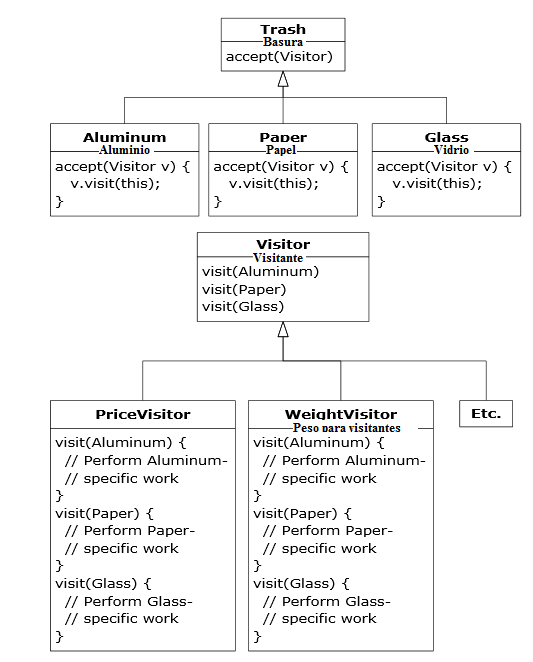
\includegraphics[width=\textwidth]{Pagna159}

Ahora, si \textbf{v} es una referencia \textbf{Visitable} para un objeto \textbf{Aluminum}, el código:    \newline

\begin{lstlisting} 
PriceVisitor pv = PriceVisitor() 
v.accept(pv) 
\end{lstlisting}

Utiliza despacho doble para causar dos llamadas a métodos polimórficos: el primero para seleccionar la versión de \textbf{Aluminum} de \textbf{accept( )}, y el segundo dentro de \textbf{accept( )} cuando la versión especifica de \textbf{visit( )} es llamada de forma dinamica usando la clase base \textbf{Visitor} con referencia \textbf{v}.         \newline

Esta configuración significa que la nueva funcionalidad puede ser añadida al sistema en forma de nuevas subclases de \textbf{Visitor}. La jerarquía \textbf{Trash} no necesita ser tocada. Este es el principal beneficio del patrón \textit{visitor}, se puede agregar nueva funcionalidad polimórfica a una jerarquía de clases sin tocar esa jerarquía (una vez que los métodos \textbf{accept( )} se han instalado). Tenga en cuenta que el beneficio es útil aquí, pero no es exactamente lo que empezamos a lograr, así que a primera vista podría decidirse que esta no es la solución deseada.      \newline

Pero mire una cosa que se ha logrado: la solución visitante Evita la clasificación de la secuencia \textbf{Trash} maestro en secuencias escritas individuales. Así, usted puede dejar todo en la única secuencia maestra y simplemente pasar a través de esa secuencia utilizando el visitante apropiado para lograr el objetivo. Aunque este comportamiento parece ser un efecto secundario del visitante, Esto proporciona lo que se requiere (evitando RTTI).       \newline

El despacho doble en el patrón \textbf{Visitor} se ocupa de determinar tanto el tipo de \textbf{Trash} como el tipo de \textbf{Visitor}. En el siguiente ejemplo, hay dos implementaciones de \textbf{Visitor: PriceVisitor} tanto para determinar y resumir el precio, y \textbf{WeightVisitor} para hacer un seguimiento de los pesos.      \newline

Se puede ver todo esto implementado en la nueva y mejorada versión del programa de reciclaje.        \newline

Al igual que con \textbf{DoubleDispatch.py}, la clase \textbf{Trash} se deja sola y una nueva interfaz es creada para agregar el método \textbf{accept( )}: \newline

\begin{lstlisting} 
# c12:trashvisitor:Visitable.py 
# An class to add visitor functionality  
# to the Trash hierarchy without  
# modifying the base class. 

class Visitable: 
  # The method: 
  def accept(self, Visitor v) 
# :~ 
\end{lstlisting}

Dado que no hay nada concreto en la clase base \textbf{Visitor}, se puede crear como una \textbf{interface}: \newline

\begin{lstlisting} 
# c12:trashvisitor:Visitor.py 
# The base class for visitors. 

class Visitor: 
  def visit(self, Aluminum a) 
  def visit(self, Paper p) 
  def visit(self, Glass g) 
  def visit(self, Cardboard c) 
# :~ 
\end{lstlisting}


\subsection*{Un decorador reflexivo}
\label{subsec:udr}
\addcontentsline{toc}{subsection}{\nameref{subsec:udr}}


En este punto, se podría seguir el mismo criterio que se utilizó para el despacho doble y crear nuevos subtipos de \textbf{Aluminum, Paper, Glass}, y \textbf{Cardboard} que implementan el método \textbf{accept( )}. Por ejemplo, el nuevo \textbf{Visitable Aluminum} se vería así: \newline

\begin{lstlisting} 
# c12:trashvisitor:VAluminum.py 
# Taking the previous approach of creating a 
# specialized Aluminum for the visitor pattern. 

class VAluminum(Aluminum)  
    implements Visitable: 
  def __init__(self, double wt): .__init__(wt)  
  def accept(self, Visitor v): 
    v.visit(self) 

# :~ 
\end{lstlisting}

Sin embargo, parece que se está enfrentando a una "explosión de interfaces:" \textbf{Trash} básico, versiones especiales para el despacho doble, y ahora las versiones más especiales para los visitantes. Claro, esta "explosión de interfaces" es arbitraria — uno podría simplemente poner los métodos adicionales de la clase \textbf{Trash}. Si se ignora que en su lugar se puede tener la oportunidad de utilizar el patrón \textit{Decorador}: parece que debería ser posible crear un \textit{Decorador} que puede ser envuelto alrededor de un objeto ordinario \textbf{Trash} y producirá la misma interfaz que \textbf{Trash} y agrega el método extra \textbf{accept( )}. De hecho, es un ejemplo perfecto del valor del \textit{Decorador}.         \newline

El doble despacho crea un problema, no obstante. Como se basa en la sobrecarga de ambos \textbf{accept( )} y \textbf{visit( )}, esto parecería requerir código especializado para cada versión diferente del método \textbf{accept( )}. Con las plantillas de C ++, esto sería bastante fácil de lograr (ya que las plantillas generan automáticamente código de tipo especializado) pero Python no tiene tal mecanismo — al menos no parece. Sin embargo, la propiedad de reflexión de Python le permite determinar la información de tipo en tiempo de ejecución, y llegar a resolver muchos problemas que parecerían requerir plantillas (aunque no tan simplemente). Aquí está el decorador que hace el truco\footnote{Esta fue una solución creada por Jaroslav Tulach en una clase de diseño de patrones que di en Praga}:       \\newpage

\begin{lstlisting} 
# c12:trashvisitor:VisitableDecorator.py 
# A decorator that adapts the generic Trash 
# classes to the visitor pattern. 
class VisitableDecorator 
extends Trash implements Visitable: 
  private Trash delegate 
  private Method dispatch 
  def __init__(self, Trash t): 
    delegate = t 
    try: 
      dispatch = Visitor.class.getMethod ( 
        "visit", Class[]: t.getClass()  
      ) 
     catch (Exception ex): 
      ex.printStackTrace() 
  def getValue(self): 
    return delegate.getValue() 
  def getWeight(self): 
    return delegate.getWeight() 
  def accept(self, Visitor v): 
    try: 
      dispatch.invoke(v, Object[]{delegate) 
     catch (Exception ex): 
      ex.printStackTrace() 
# :~ 
\end{lstlisting}

[[Descripción del uso de Reflexión]]  \newline

La única otra herramienta que necesitamos es un nuevo tipo de adaptador \textbf{Fillable} que automáticamente decora los objetos a medida que se crean a partir del archivo original \textbf{Trash.dat}. Pero esto bien podría ser un decorador de sí mismo, la decoración de cualquier tipo de \textbf{Fillable}:        \newline

\begin{lstlisting} 
# c12:trashvisitor:FillableVisitor.py  
# Adapter Decorator that adds the visitable  
# decorator as the Trash objects are  
# being created. 

class FillableVisitor 
implements Fillable: 
  private Fillable f 
  def __init__(self, Fillable ff): f = ff  
  def addTrash(self, Trash t): 
    f.addTrash(VisitableDecorator(t)) 
# :~ 
\end{lstlisting}
Ahora se puede envolver alrededor de cualquier tipo de \textbf{Fillable} existente,  o cualquier otros nuevos que aún no se han creado. \newline

El resto del programa crea tipos \textbf{Visitor} específicos y los envía a través de una lista única de objetos \textbf{Trash}:   \newline

\begin{lstlisting} 
# c12:trashvisitor:TrashVisitor.py  
# The "visitor" pattern with VisitableDecorators. 

# Specific group of algorithms packaged 
# in each implementation of Visitor: 
class PriceVisitor(Visitor): 
  private double alSum # Aluminum 
  private double pSum # Paper 
  private double gSum # Glass 
  private double cSum # Cardboard 
  def visit(self, Aluminum al): 
    double v = al.getWeight() * al.getValue() 
    print "value of Aluminum= " + v 
    alSum += v 
    
  def visit(self, Paper p): 
    double v = p.getWeight() * p.getValue() 
    print "value of Paper= " + v 
    pSum += v 
    
  def visit(self, Glass g): 
    double v = g.getWeight() * g.getValue() 
    print "value of Glass= " + v 
    gSum += v 
    
  def visit(self, Cardboard c): 
    double v = c.getWeight() * c.getValue() 
    print "value of Cardboard = " + v 
    cSum += v 
    
  def total(self): 
    print ( 
      "Total Aluminum: $" + alSum + 
      "\n Total Paper: $" + pSum +  
      "\nTotal Glass: $" + gSum +  
      "\nTotal Cardboard: $" + cSum + 
      "\nTotal: $" +  
        (alSum + pSum + gSum + cSum)) 
        
class WeightVisitor(Visitor): 
  private double alSum # Aluminum 
  private double pSum # Paper 
  private double gSum # Glass 
  private double cSum # Cardboard 
  
  def visit(self, Aluminum al): 
    alSum += al.getWeight() 
    print ("weight of Aluminum = " 
        + al.getWeight()) 
        
  def visit(self, Paper p): 
    pSum += p.getWeight() 
    print ("weight of Paper = " 
        + p.getWeight()) 
        
  def visit(self, Glass g): 
    gSum += g.getWeight() 
    print ("weight of Glass = " 
        + g.getWeight()) 
        
  def visit(self, Cardboard c): 
    cSum += c.getWeight() 
    print ("weight of Cardboard = " 
        + c.getWeight()) 
        
  def total(self): 
    print ( 
      "Total weight Aluminum: "  + alSum + 
      "\nTotal weight Paper: " + pSum + 
      "\nTotal weight Glass: " + gSum + 
      "\nTotal weight Cardboard: " + cSum + 
      "\nTotal weight: " +  
        (alSum + pSum + gSum + cSum))
        
class TrashVisitor(UnitTest): 
  Collection bin = ArrayList() 
  PriceVisitor pv = PriceVisitor() 
  WeightVisitor wv = WeightVisitor() 
  def __init__(self): 
    ParseTrash.fillBin("../trash/Trash.dat",  
      FillableVisitor( 
        FillableCollection(bin))) 
        
  def test(self): 
    Iterator it = bin.iterator() 
    while(it.hasNext()): 
      Visitable v = (Visitable)it.next() 
      v.accept(pv) 
      v.accept(wv) 
      
    pv.total() 
    wv.total() 
    
  def main(self, String args[]): 
    TrashVisitor().test() 
    
# :~ 
\end{lstlisting}

En \textbf{Test( )}, se observa cómo se añade la visitabilidad simplemente creando un tipo diferente de contenedor usando el decorador. Se observa también que el adaptador \textbf{FillableCollection} tiene la apariencia de ser utilizado como decorador (para \textbf{ArrayList}) en esta situación.  Ahora bien, cambia completamente la interfaz del \textbf{ArrayList}, visto que la definición de \textit{Decorador} es que la interfaz de la clase decorada aún debe estar allí después de la decoración.      \newline

Tenga en cuenta que la forma del código del cliente (que se muestra en la clase \textbf{Test}) ha cambiado de nuevo, a partir de los enfoques originales al problema. Ahora sólo hay un solo contenedor \textbf{Trash}. Los dos objetos \textbf{Visitor} son aceptados en cada elemento de la secuencia, y realizan sus operaciones. Los visitantes mantienen sus propios datos internos para concordar los pesos y los precios totales.        \newline

Finalmente, allí no hay identificación de tipo en tiempo de ejecución que no sea emitido a \textbf{Trash} cuando se sacan cosas fuera de la secuencia. Esto, también, podría ser eliminado con la implementación de tipos parametrizados en Java.        \newline

Una manera de distinguir esta solución de la solución de despacho doble descrita anteriormente, es tener en cuenta que, en la solución del doble despacho, solamente uno de los métodos sobrecargados, \textbf{add( )},  fue anulado cuando se creó cada subclase, mientras que aquí cada uno de los métodos \textbf{visit( )} sobrecargados es anulado en cada subclase de \textbf{Visitor}.          \newline

\subsubsection*{¿Más acoplamiento?}
\label{subsubsec:moreA}
\addcontentsline{toc}{subsubsection}{\nameref{subsubsec:moreA}}


Hay mucho más código aquí, y hay acoplamiento definitivo entre la jerarquía \textbf{Trash} y la jerarquía \textbf{Visitor}. Ahora bien, también hay alta cohesión dentro de los respectivos conjuntos de clases: cada uno de ellos hacen una sola cosa (\textbf{Trash} describe Basura, mientras que \textbf{Visitor} describe las acciones realizadas en \textbf{Trash}), que es un indicador de un buen diseño. Claro, en este caso funciona bien sólo si está agregando nuevos \textbf{Visitor}s, pero esto se obtiene en el camino cuando se agregan nuevos tipos de \textbf{Trash}.          \newline

Bajo acoplamiento entre clases y alta cohesión dentro de una clase es sin duda un objetivo de diseño importante. Aplicado sin pensar, sin embargo, puede impedirle el logro de un diseño más elegante. Parece que algunas clases, inevitablemente, tienen una cierta intimidad entre ellas. Estos a menudo ocurren en parejas que quizás podrían ser llamados \textit{couplets : coplas}; por ejemplo, los contenedores y los iteradores. El par anterior \textbf{Trash-Visitor} parece ser otro de tipo \textit{couplet}.    \newline

\subsection*{¿RTTI considerado dañino?}
\label{subsec:rtticd}
\addcontentsline{toc}{subsection}{\nameref{subsec:rtticd}}

Varios diseños en este capítulo intentan eliminar RTTI, lo cual podría darle la impresión de que se “considera perjudicial" (la condena utilizado para pobres, el malogrado \textbf{goto}, que por lo tanto nunca fue puesto en Java). Esto no es verdad; es el mal uso de RTTI, ese es el problema. La razón por la que nuestros diseños eliminan RTTI se debe a la mala aplicación de esa característica que impide extensibilidad, mientras que el objetivo expresado era poder añadir un nuevo tipo al sistema con el menor impacto alrededor del código como sea posible. Dado que RTTI es a menudo mal usado por tener que buscar cada tipo en su sistema, provoca que el código que no sea extensible: cuando se agrega un nuevo tipo, se tiene que ir a buscar por todo el código en el que se usa RTTI, y si se pierde alguno, no se conseguirá ayuda del compilador.     \newline

Sin embargo, RTTI no crea automáticamente el código no extensible. Vamos a revisar el reciclador de basura una vez más. Esta vez, una nueva herramienta será introducida, la cual yo llamo un \textbf{TypeMap}. Este contiene un \textbf{HashMap} que contiene \textbf{ArrayList}s, pero la interfaz es simple: se puede agregar \textbf{add( )} como un nuevo objeto, y \textbf{get( )} como un \textbf{ArrayList} que contiene todos los objetos de un tipo particular. Las claves para el contenido \textbf{HashMap} son los tipos en el \textbf{ArrayList} asociado. La belleza de este diseño (sugerido por Larry O'Brien) es que el \textbf{TypeMap} agrega dinámicamente un nuevo par cada vez que encuentra un nuevo tipo, por lo que cada vez que añade un nuevo tipo al sistema (incluso si se agrega el nuevo tipo en tiempo de ejecución), se adapta.  \newline

Nuestro ejemplo  nuevamente se basará en la estructura de los tipos \textbf{Trash} en \textbf{package c12.Trash} (y el archivo \textbf{Trash.dat} utilizado se pueden utilizar aquí sin modificar):        \newline

\begin{lstlisting} 
# c12:dynatrash:DynaTrash.py  
# Using a Map of Lists and RTTI 
# to automatically sort trash into 
# ArrayLists. This solution, despite the 
# use of RTTI, is extensible. 

# Generic TypeMap works in any situation: 
class TypeMap: 
  private Map t = HashMap() 
  def add(self, Object o): 
    Class type = o.getClass() 
    if(t.has_key(type)) 
      ((List)t.get(type)).add(o) 
    else: 
      List v = ArrayList() 
      v.add(o) 
      t.put(type,v) 
      
  def get(self, Class type): 
    return (List)t.get(type) 
    
  def keys(self):  
    return t.keySet().iterator()  
    
# Adapter class to allow callbacks 
# from ParseTrash.fillBin(): 
class TypeMapAdapter(Fillable): 
  TypeMap map 
  def __init__(self, TypeMap tm): map = tm  
  def addTrash(self, Trash t): map.add(t)  
  
class DynaTrash(UnitTest): 
  TypeMap bin = TypeMap() 
  
    def __init__(self): 
    ParseTrash.fillBin("../trash/Trash.dat",  
      TypeMapAdapter(bin)) 
      
  def test(self): 
    Iterator keys = bin.keys() 
    while(keys.hasNext()) 
      Trash.sumValue( 
        bin.get((Class)keys.next()).iterator())
        
  def main(self, String args[]): 
    DynaTrash().test() 
# :~ 
\end{lstlisting}

Aunque potente, la definición para \textbf{TypeMap} es simple. Contiene un \textbf{HashMap}, y el método \textbf{add( )} hace la mayoría del trabajo. Cuando se agrega un nuevo objeto \textbf{add( )}, se extrae la referencia para el objeto \textbf{Class} para ese tipo. Esto se utiliza como una clave para determinar si un \textbf{ArrayList} que sostiene objetos de ese tipo ya está presente en el \textbf{HashMap}. Si es así, ese \textbf{ArrayList} se extrae y el objeto se añade al \textbf{ArrayList}. Si no, el objeto \textbf{Class} y un nuevo \textbf{ArrayList} se añaden como un par clave-valor.       \newline

Se puede obtener un \textbf{Iterator} de todos los objetos \textbf{Class} de   \textbf{keys( )}, y usar cada objeto \textbf{Class} para buscar el correspondiente \textbf{ArrayList} con \textbf{get( )}. Y eso es todo lo que hay que hacer.         \newline

El método \textbf{filler( )} es interesante porque se aprovecha del diseño de \textbf{ParseTrash.fillBin( )},  que no sólo tratar de llenar un \textbf{ArrayList} sino cualquier cosa que implementa la interfaz \textbf{Fillable} con su método \textbf{addTrash( )}.  Todo \textbf{filler( )} necesita hacer es devolver una referencia a una \textbf{interface} que implementa \textbf{Fillable}, y luego esta referencia puede ser utilizado como un argumento a \textbf{fillBin( )} como esto:    \newline

\begin{lstlisting} 
ParseTrash.fillBin("Trash.dat", bin.filler()) 
\end{lstlisting}

Para producir esta referencia, una \textit{clase interna anónima} (descrito en el capítulo 8 de \textit{Thinking in Java}, segunda edición) es utilizada. Nunca se necesita un llamado a la clase para implementar \textbf{Fillable}, sólo necesita una referencia a un objeto de esa clase, por lo que este es un uso apropiado de las clases internas anónimas. \newline

Una cosa interesante sobre este diseño es que a pesar de que no fue creado para manejar la clasificación, \textbf{fillBin( )} está realizando una clasificación cada vez que se inserta un objeto \textbf{Trash} dentro de \textbf{bin}.        \newline

Gran parte de \textbf{class DynaTrash} debería estar familiarizado a partir de los ejemplos anteriores. Esta vez, en lugar de colocar los nuevos objetos \textbf{Trash} en un \textbf{bin} de tipo \textbf{ArrayList}, \textbf{bin} es de tipo \textbf{TypeMap}, así que cuando la basura es arrojada en \textbf{bin} se ordena de inmediato por el \textbf{TypeMap} del mecanismo de clasificación interna. Dando un paso a través de \textbf{TypeMap} y operando en cada \textbf{ArrayList} individual se convierte en un asunto sencillo.  \newline

Como puede ver, la adición de un nuevo tipo al sistema no afectará este código en absoluto, y el código en \textbf{TypeMap} es completamente independiente. Esta es ciertamente la solución más pequeña del problema, y podría decirse que el más elegante también. No depende mucho de de RTTI, pero observe que cada par clave-valor en el \textbf{HashMap} está en busca de un solo tipo. En adición, no hay manera que se pueda "olvidar" añadir el código adecuado a este sistema cuando se agrega un nuevo tipo, ya que no hay ningún código que necesite agregar.       \newline

\subsection*{Resumen}
\label{subsec:Resumen}
\addcontentsline{toc}{subsection}{\nameref{subsec:Resumen}}

Surgir %aparecer, subir
con un diseño como \textbf{TrashVisitor.py} que contiene una gran cantidad de código que los diseños anteriores puede parecer en un principio ser contraproducente. Vale la pena notar lo que estás tratando de lograr con varios diseños. Los patrones de diseño en general se esfuerzan por \textit{separar las cosas que cambian de las cosas que permanecen igual}. Las "cosas que cambian" puede referirse a muchos tipos diferentes de cambios. Quizás el cambio ocurre porque el programa se coloca en un nuevo entorno o porque algo en el entorno actual cambia: (esto podría ser: "El usuario quiere añadir una nueva forma para el diagrama actualmente en la pantalla"). O, como en este caso, el cambio podría ser la evolución del cuerpo del código. Mientras que las versiones anteriores del ejemplo de clasificación de basura enfatizaron la adición de nuevos tipos de \textbf{Trash} al sistema, \textbf{TrashVisitor.py} le permite añadir fácilmente nuevas funcionalidades sin molestar a la jerarquía \textbf{Trash}. Hay más código en \textbf{TrashVisitor.py}, pero la adición de nueva funcionalidad para \textbf{Visitor} es de mal gusto. Si esto es algo que sucede a menudo, entonces vale la pena el esfuerzo extra y el código para hacer que suceda con más facilidad. \newline

El descubrimiento del vector de cambio no es un asunto trivial; esto no es algo que un analista usualmente puede detectar cuando el programa esté en la etapa del diseño inicial. La información necesaria probablemente no aparecerá hasta las últimas fases del proyecto: a veces sólo en las fases de diseño o de implementación se descubre una necesidad más profunda o más sutil en su sistema. En el caso de la adición de nuevos tipos (el cual fue el foco de la mayoría de los ejemplos "reciclar") se puede dar cuenta de que se necesita una jerarquía de herencia particular sólo cuando se está en la fase de mantenimiento y de inicio en la ampliación del sistema! \newline

Una de las cosas más importantes que aprenderá mediante el estudio de los patrones de diseño parece ser  un cambio de actitud de lo que se ha promovido hasta ahora en este libro. Es decir: "Programación Orientada a Objetos es todo acerca de polimorfismo." Esta declaración puede producir el síndrome "dos años meceando, con un martillo"  (todo se ve como un clavo). Dicho de otra manera, es bastante difícil "obtener" polimorfismo, y una vez que lo hace, trate de emitir  % ==moldear== cast
todos sus diseños en un molde particular.\newline

¿Qué patrones de diseño dicen que la Programación Orientada a Objetos no se trata sólo de polimorfismo?. Esto se trata de "la separación de cosas que cambian y de las cosas que permanecen igual." El Polimorfismo es una manera especialmente importante para hacer esto, y resulta ser útil si el lenguaje de programación apoya directamente el polimorfismo (por lo que no se tienen que conectar por el programador, lo que lo haría prohibitivamente caro). Pero los patrones de diseño en general muestran otras maneras de lograr el objetivo básico, y una vez que se ha entendido esto, comenzarán a surgir diseños más creativos.\newline

Desde que el libro \textit{Design Patterns} salió e hizó tal impacto, la gente ha estado buscando otros patrones. Se puede ver más de ellos aparecer con el paso del tiempo. Estos son algunos sitios recomendados por by Jim Coplien, de fama C ++ (\textit{http://www.bell-labs.com/~cope}), que es uno de los principales promotores del movimiento de los patrones:      \newline

\textit{http://st-www.cs.uiuc.edu/users/patterns \newline
http://c2.com/cgi/wiki \newline
http://c2.com/ppr  \newline
http://www.bell-labs.com/people/co \newline
pe/Patterns/Process/index.html  \newline
http://www.bell-labs.com/cgi-user/OrgPatterns/OrgPatterns  \newline
http://st-www.cs.uiuc.edu/cgi-bin/wikic/wikic  \newline
http://www.cs.wustl.edu/~schmidt/patterns.html  \newline
http://www.espinc.com/patterns/overview.html } \newline

También tenga en cuenta que ha habido una conferencia anual sobre los patrones de diseño, llamada PLOP, que produce unas actas publicadas, la tercera de las cuales salieron a finales de 1997 (todas publicadas por Addison-Wesley).   \newline

\subsection*{Ejercicios}
\label{subsec:Ejercicios14}
\addcontentsline{toc}{subsection}{\nameref{subsec:Ejercicios14}}

\begin{enumerate}
    
    \item Añadir la clase \textbf{Plastic} a \textbf{TrashVisitor.py}
    \item Agregar la clase \textbf{Plastic} a \textbf{DynaTrash.py}
    \item Crear un decorador como \textbf{VisitableDecorator}, pero para el ejemplo de despacho múltiple, junto con una clase "decorador adaptador " como la creada para \textbf{VisitableDecorator}. Construir el resto del ejemplo y demostrar que funciona.
    
\end{enumerate}